\documentclass[12pt,twoside]{article}
\usepackage{mathtools} % for DeclareParedDelimiter
\usepackage{listings}
\usepackage{graphicx} % Required for including images
\newcommand{\reporttitle}{Foundations of Machine Learning}
\newcommand{\reportauthor}{Lionel Ngoupeyou Tondji}
\newcommand{\reporttype}{Assignment: Statistics and Probability}
\newcommand\myeq{\mathrel{\overset{\makebox[0pt]{\mbox{\normalfont\tiny\sffamily iid}}}{=}}}





\begin{document}
% front page

% Last modification: 2016-09-29 (Marc Deisenroth)
\begin{titlepage}
\newcommand{\HRule}{\rule{\linewidth}{0.5mm}} % Defines a new command for the horizontal lines, change thickness here


%----------------------------------------------------------------------------------------
%	LOGO SECTION
%----------------------------------------------------------------------------------------

\begin{center}

\includegraphics[height = 2cm]{qla}\hspace{4mm}

\includegraphics[height=2cm]{aims-rwanda}
\end{center}
 

\begin{center} % Center remainder of the page

%----------------------------------------------------------------------------------------
%	HEADING SECTIONS
%----------------------------------------------------------------------------------------
\textsc{\LARGE \reporttype}\\[1.5cm] 
\textsc{\Large African Institute for Mathematical Sciences}\\[0.5cm] 
\textsc{\large Quantum Leap Africa}\\[0.5cm] 
%----------------------------------------------------------------------------------------
%	TITLE SECTION
%----------------------------------------------------------------------------------------

\HRule \\[0.4cm]
{ \huge \bfseries \reporttitle}\\ % Title of your document
\HRule \\[1.5cm]
\end{center}
%----------------------------------------------------------------------------------------
%	AUTHOR SECTION
%----------------------------------------------------------------------------------------

\begin{minipage}{0.4\hsize}
 \begin{flushleft} \large
 \textit{Author: Lionel Ngoupeyou Tondji}\\
 \end{flushleft}
  \vspace{2cm}
 \makeatletter
 Date: \@date 
\end{minipage}
\vfill % Fill the rest of the page with whitespace



\makeatother

\end{titlepage}




\section{Discrete Models}
\subsection*{c)} The following graph is showing the evidence for each model
\begin{center}
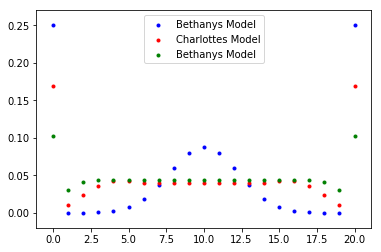
\includegraphics{../scatter}     
\end{center}

\subsection*{d)}
\subsubsection*{1)}
Table over the 11 different possibilities under each model \\ \\.
\begin{tabular}{|c|c|c|}
	\hline 
	Bethany-model & Charlotte-model & Davina-model \\ 
	\hline 
0	& 0.00000000e+00 & 0.00000000e+00 \\ 
	\hline 
0	& 0.00000000e+00 & 7.78633801e-09\\ 
	\hline 
0	&  5.66695902e-05 & 2.79676219e-05 \\ 
	\hline 
0	& 0.00000000e+00 & 2.13746139e-03 \\ 
	\hline 
0	& 6.19681968e-02 & 3.05825945e-02 \\ 
	\hline 
1	& 0.00000000e+00 & 1.55251489e-01 \\ 
	\hline 
0	& 7.05856492e-01 & 3.48354866e-01 \\ 
	\hline 
0	& 0.00000000e+00 & 3.44952256e-01 \\ 
	\hline 
0	& 2.32118641e-01 & 1.14555379e-01 \\ 
	\hline 
0	& 0.00000000e+00 & 4.13797926e-03 \\ 
	\hline 
0	& 0.00000000e+00 & 0.00000000e+00 \\ 
	\hline 
\end{tabular} 

\subsubsection*{2)} Predictive distribution \\\\
\begin{tabular}{|c|c|c|}
	\hline 
	Bethany-model & Charlotte-model & Davina-model \\ 
	\hline 
	0.5 & 0.63400742105992502 & 0.63635359808933689 \\ 
	\hline 
\end{tabular} 

\subsection*{e)}
\subsubsection*{1)} According to the question $c)$ we can say that all of the three girls are right because the graph is in accord with what they have said at the beginning.

\subsubsection*{2)} What happen If Andrew had drawn 130 white balls out of 200?\\ 
\begin{center}
	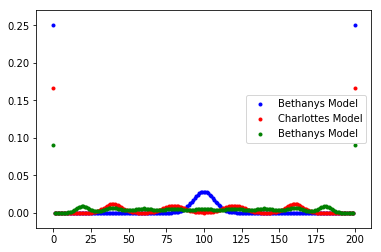
\includegraphics{../index1}     
\end{center}
As we can see on the graph, when $nTotal$ is very big the Charlotte's model and the Bethany's model tends to be the same.


\section{Continuous Models}
\subsection*{a)} Derive Fred’s maximum likelihood solution for the parameters of his model.
The parameters for the Fred's model is $\theta = (\mu, \sigma^2)$.\\
Likelihood: Probability of the observed data x given the parameters $\theta$\\

The Likelihood is given by :
\begin{equation*}
p(x| \theta) = p(x_1,x_2,....., x_N\ \theta) = \prod_{n=1}^{N} p(x_n| \theta)
\end{equation*}

Our goal is to Find the parameters that maximize the likelihood $p(x| \theta)$.\\
The step of finding the maximum are :
\begin{itemize}
	\item  Compute gradient with respect to θ
	\item  Set gradient to 0
	\item  Solve for θ
\end{itemize}

So we have :
\begin{equation*}
p(x| \theta) = \prod_{n=1}^{N} p(x_n| \theta) = \prod_{n=1}^{N} \mathcal{N}(x_n| \mu, \sigma^2)
\end{equation*}

But instead of maximizing the Likelihood, we will maximize the log-Likelihood because log is a strictly monotonically function increasing function.

Why are we allow to this transformation? because
\begin{itemize}
	\item  We will obtain The same maximum
	\item  Gradients easy
	\item  Fewer numerical problems
\end{itemize}

Thus, the Log Likelihood is given by :
\begin{align*}
log \,p(x| \theta) &= log \, \prod_{n=1}^{N} p(x_n| \theta) \\
				   &= \sum_{n=1}^{N} log \, \left( \frac{1}{\sqrt{2 \pi \sigma^2}} exp\big(-\frac{1}{2 \sigma^2}\big(x_n - \mu\big)^2\big) \right) \\
				   &= -\frac{N}{2} log\big(2 \pi \sigma^2\big) + \sum_{n=1}^{N}  \, \left( -\frac{1}{2 \sigma^2}\big(x_n - \mu\big)^2 \right) \\
\end{align*}

The gradient of the Log Likelihood with respect to $\mu$ is given by :
\begin{align*}
\frac{\partial}{\partial \mu}log \,p(x| \theta) &= \frac{\partial}{\partial \mu}  \left( -\frac{N}{2} log\big(2 \pi \sigma^2\big) + \sum_{n=1}^{N}  \, \left( -\frac{1}{2 \sigma^2}\big(x_n - \mu\big)^2 \right) \right) \\
&= \sum_{n=1}^{N}  \, \frac{\partial}{\partial \mu} \left(-\frac{1}{2 \sigma^2}\big(x_n - \mu\big)^2  \right)  \\
&= \sum_{n=1}^{N}  \, \left(\frac{1}{\sigma^2}\big(x_n - \mu\big) \right) \\
\end{align*}

Setting the gradient that we compute before to zero, we obtain:
\begin{equation*}
\sum_{n=1}^{N}  \, \left(\frac{1}{\sigma^2}\big(x_n - \mu\big) \right) = 0 \\
\Longrightarrow  \sum_{n=1}^{N}  \,x_n - N \mu = 0
\end{equation*}

So we obtain :
\begin{equation}
\boxed{ \mu _{ML} = \frac{1}{N} \sum_{n=1}^{N} x_n }
\end{equation}

Let pose $\alpha = \sigma^2$.\\
The gradient of the Log Likelihood with respect to $\sigma ^2$ is given by :
\begin{align*}
\frac{\partial}{\partial \alpha}log \,p(x| \theta) &= \frac{\partial}{\partial \alpha}  \left( -\frac{N}{2} log\big(2 \pi \alpha \big) + \sum_{n=1}^{N}  \, \left( -\frac{1}{2 \alpha}\big(x_n - \mu\big)^2 \right) \right) \\
&= \frac{\partial}{\partial \alpha}  \left( -\frac{N}{2} log\big(2 \pi \alpha \big)\right) + \frac{\partial}{\partial \alpha}  \left( \sum_{n=1}^{N}  \, \left( -\frac{1}{2 \alpha}\big(x_n - \mu\big)^2 \right) \right) \\
&= -\frac{N}{2 \alpha} + \sum_{n=1}^{N}  \,  \frac{1}{2 \alpha^2}\big(x_n - \mu\big)^2  \\
\end{align*}

Setting the gradient that we compute before to zero, we obtain:
\begin{equation*}
-\frac{N}{2 \alpha} + \sum_{n=1}^{N}  \,  \frac{1}{2 \alpha^2}\big(x_n - \mu\big)^2  = 0 \\
\Longrightarrow  -N \alpha + \sum_{n=1}^{N}  \,  \big(x_n - \mu\big)^2  = 0
\end{equation*}

Replacing $\alpha$ by $\sigma^2$

\begin{equation*}
-N \sigma^2 + \sum_{n=1}^{N}  \,  \big(x_n - \mu\big)^2  = 0
\end{equation*}

So we obtain :
\begin{equation}
\boxed{ \sigma^2 _{ML} = \frac{1}{N} \sum_{n=1}^{N}  \,  \big(x_n - \mu\big)^2}
\end{equation}
\subsection*{b)} Using only the properties of expectation and variance of linear combinations of iid random variables, show that the maximum likehood estimator $\sigma^2 _{ML}$ is biased. (that is, taking the expectation of the maximum likelihood estimator with respect $\mathcal{N}(\mu, \sigma^2)$ does not return $\sigma^2$ ).\\ \\

From the previous question, we already have the value of $\sigma^2 _{ML}$
\begin{align*}
\sigma^2 _{ML} &= \frac{1}{N} \sum_{n=1}^{N}  \,  \big(x_n - \mu\big)^2 \\
               &= \frac{1}{N} \sum_{n=1}^{N}  \,  \big(x_n - \mu_{ML}\big)^2 \\
               &= \frac{1}{N} \sum_{n=1}^{N}  \,  x_n^2 - \frac{2}{N} \sum_{n=1}^{N}  \, x_n \mu_{ML}  + \mu_{ML}^2 \\
               &= \frac{1}{N} \sum_{n=1}^{N}  \,  x_n^2 -  2 \mu_{ML} \left( \frac{1}{N} \sum_{n=1}^{N}  \, x_n \right)   + \mu_{ML}^2 \\
               &= \frac{1}{N} \sum_{n=1}^{N}  \,  x_n^2 -  2 \mu_{ML}^2 + \mu_{ML}^2 \\
               &= \frac{1}{N} \sum_{n=1}^{N}  \,  x_n^2  - \mu_{ML}^2 \\
\end{align*}

Now we can compute the expectation $\sigma^2 _{ML}$:
\begin{align*}
E(\sigma^2 _{ML}) &= E\left(\frac{1}{N} \sum_{n=1}^{N}  \,  x_n^2  - \mu_{ML}^2 \right) \\
&= E \left(\frac{1}{N} \sum_{n=1}^{N}  \,  x_n^2 \right)  - E(\mu_{ML}^2) \\
&= \frac{1}{N} \sum_{n=1}^{N} E(x_n^2)  - E(\mu_{ML}^2) \\
& \myeq  E(x_N^2) - E(\mu_{ML}^2) \\
\end{align*}

According to the alternative definition of variance, $\sigma_x = E(x^2) - E(x)^2$ and similarly, $\sigma_{\mu_{ML}} = E(x_{\mu_{ML}}^2) - E(x_{\mu_{ML}})^2$ where the random variable is $\mu_{ML}.$ We can notice that $E(x) = E(x_{\mu_{ML}}) = \mu$. Plug the 2 equations to the
derivation:
\begin{align*}
E(\sigma^2 _{ML})  &= (\sigma_x^2 + \mu^2) - (\sigma_{\mu_{ML}}^2 + \mu^2) \\
                   &= \sigma_x^2  - \sigma_{\mu_{ML}}^2  \\
\end{align*}

We have : 
\begin{align*}
\sigma_{\mu_{ML}}^2 &= Var(\frac{1}{N} \sum_{n=1}^{N} x_n) \\
                    &= \frac{1}{N^2}Var( \sum_{n=1}^{N} x_n) \\
                    & \myeq \frac{1}{N^2} \sum_{n=1}^{N} Var( x_n) \\
                    &= \frac{1}{N^2} \sum_{n=1}^{N} \sigma_x^2 \\
                    &= \frac{1}{N} \sigma_x^2 \\
\end{align*}

Plug back to the $E(\sigma^2 _{ML})$ derivation,

So we have : 
\begin{align*}
E(\sigma^2 _{ML}) &= \sigma_x^2  - \sigma_{\mu_{ML}}^2   \\
                  &= \sigma_x^2 - \frac{1}{N} \sigma_x^2\\
                  &= \frac{N-1}{N} \sigma_x^2\\
\end{align*}



So we get :
\begin{equation}
E(\sigma^2 _{ML}) \neq \sigma^2 _{ML}
\end{equation}

Then we conclude that the estimator $\sigma^2 _{ML}$ is biased.\\ \\

\subsection*{c)} Derive the MAP solution for μ in George’s model. Do your analysis replacing 10 with $\mu_0$ and 25 with $\sigma_0^2$ (this makes it easier to read). Write your answer in terms of Fred’s maximum likelihood solution $\mu_{ML}$.\\ \\

The Posterior is given by :
\begin{equation*}
p(\theta|x) = \frac{p(x|\theta)p(\theta)}{p(x)}
\end{equation*}

Where $x =(x_1,x_2,....,x_n)$ , $x \sim \mathcal{N}(\mu, \sigma^2)$ and $\mu \sim \mathcal{N}(\mu_0, \sigma^2_o)$

Our goal is to Find the parameters that maximize the log-Posterior $p(\theta|x)$.\\
The step of finding the maximum are :
\begin{itemize}
	\item  Compute gradient with respect to θ
	\item  Set gradient to 0
	\item  Solve for θ
\end{itemize}

Thus, the Log Posterior is given by :
\begin{align*}
log \, p(\theta|x) &= log \, p(x|\theta) + log \, p(\theta) + cste \\
                   &= -\frac{N}{2} log\big(2 \pi \sigma^2\big) - \sum_{n=1}^{N}  \, \left( \frac{1}{2 \sigma^2}\big(x_n - \mu\big)^2 \right) + log \, \mathcal{N}(\mu_0, \sigma_0^2)\\
                   &= -\frac{N}{2} log\big(2 \pi \sigma^2\big) - \sum_{n=1}^{N}  \, \left( \frac{1}{2 \sigma^2}\big(x_n - \mu\big)^2 \right)  -\frac{1}{2} log\big(2 \pi \sigma_0^2\big) - \left( \frac{1}{2 \sigma_0^2}\big(\mu - \mu_0\big)^2 \right) \\
\end{align*}

The gradient of the Log Posterior with respect to $\mu$ is given by :
\begin{align*}
\frac{\partial}{\partial \mu}log \,p(\theta|x) &= \frac{\partial}{\partial \mu}  \left( -\frac{N}{2} log\big(2 \pi \sigma^2\big) - \sum_{n=1}^{N}  \, \left( \frac{1}{2 \sigma^2}\big(x_n - \mu\big)^2 \right)  -\frac{1}{2} log\big(2 \pi \sigma_0^2\big) - \left( \frac{1}{2 \sigma_0^2}\big(\mu - \mu_0\big)^2 \right) \right) \\
&= \sum_{n=1}^{N}  \, \left( \frac{1}{\sigma^2}\big(x_n - \mu\big) \right)  -\frac{1}{\sigma_0^2}\big(\mu - \mu_0\big) \\
\end{align*}

Setting this gradient that we compute before to zero, we obtain:
\begin{equation*}
\frac{\partial}{\partial \mu}log \,p(\theta|x) = 0 \Longrightarrow \sum_{n=1}^{N}  \, \left( \frac{1}{\sigma^2}\big(x_n - \mu\big) \right) -\frac{1}{\sigma_0^2}\big(\mu - \mu_0\big) = 0 
\end{equation*}

\begin{equation*}
\Longrightarrow \sum_{n=1}^{N}  \, \frac{1}{\sigma^2} x_n - \frac{N}{\sigma^2} \mu  -\frac{1}{\sigma_0^2}\mu + \frac{1}{\sigma_0^2} \mu_0 = 0
\end{equation*}

\begin{equation*}
\Longrightarrow \frac{N}{\sigma^2} \mu_{ML} - \frac{N}{\sigma^2} \mu  -\frac{1}{\sigma_0^2}\mu + \frac{1}{\sigma_0^2} \mu_0 = 0
\end{equation*}

\begin{equation*}
\Longrightarrow \mu \left(\frac{N}{\sigma^2} + \frac{1}{\sigma_0^2} \right) = \frac{N}{\sigma^2} \mu_{ML} + \frac{1}{\sigma_0^2} \mu_0
\end{equation*}

So we obtain :
\begin{equation}
\boxed{ \mu_{MAP} = \frac{1}{\left(\frac{N}{\sigma^2} + \frac{1}{\sigma_0^2} \right)} \left( \frac{N}{\sigma^2} \mu_{ML} + \frac{1}{\sigma_0^2} \mu_0 \right) }
\end{equation}

\subsection*{d)} Explaining your reasoning, calculate the posterior for George’s model. Show that the MAP point you calculated in the previous exercise is also the mean, and give a reason why this is true in this example but not true in general. Again use $\mu_0$ and $\sigma_0^2$ rather than use the actual numbers.

The Posterior is given by :
\begin{equation*}
p(\theta|x) = \frac{p(x|\theta)p(\theta)}{p(x)}
\end{equation*}

Where $x =(x_1,x_2,....,x_n)$ , $x \sim \mathcal{N}(\theta, \sigma^2)$ and $\theta \sim \mathcal{N}(\mu_0, \sigma^2_0)$.

Given the formula for the posterior we can say that : 
\begin{equation*}
p(\theta|x) \propto p(x|\theta)p(\theta)
\end{equation*}

We get :
\begin{equation*}
p(x|\theta)p(\theta) = e^{-\frac{1}{2}M}
\end{equation*}

Where :
\begin{align*}
M &= \sum_{n=1}^{N} \frac{1}{\sigma^2}(x_n - \theta)^2 + \frac{1}{\sigma^2_0}(\theta - \mu_0)^2 \\
  &= \frac{1}{\sigma^2} \sum_{n=1}^{N}x_n^2 + \frac{N}{\sigma^2} \theta^2 - \frac{2\theta}{\sigma^2}\sum_{n=1}^{N}x_n + \frac{\theta^2}{\sigma_0^2} + \frac{\mu_0^2}{\sigma_0^2} - \frac{2\theta\mu_0}{\sigma_0^2}\\
  &= \underbrace{ \left(\frac{N}{\sigma^2} + \frac{1}{\sigma_0^2}\right)}_a\theta^2 - 2\underbrace{ \left(\frac{1}{\sigma^2}\sum_{n=1}^{N}x_n + \frac{\mu_0}{\sigma_0^2} \right)}_b\theta + \underbrace{\left(\frac{1}{\sigma^2} \sum_{n=1}^{N}x_n^2 + \frac{\mu_0^2}{\sigma_0^2} \right)}_c
\end{align*}

So :
\begin{align*}
M &= a \theta^2 - 2b \theta + c \\
  &= a \left(\theta^2 - \frac{2b}{a} + \frac{c}{a}\right) \\
  &= a \left[\left( \theta - \frac{b}{a} \right)^2 - \frac{b^2}{a^2} + \frac{c}{a}\right] \\
  &= a \left( \theta - \frac{b}{a} \right)^2 - \frac{b^2}{a} + c
\end{align*}

Then :
\begin{align*}
p(x|\theta)p(\theta) &= exp \left[-\frac{1}{2}\left(a ( \theta - \frac{b}{a} )^2 - \frac{b^2}{a} + c\right)\right] \\
                     &= Cste \times exp \left(-\frac{1}{2}a( \theta - \frac{b}{a} )^2\right)
\end{align*}
We  can conclude that $p(\theta|x) \sim \mathcal{N}(\frac{b}{a}, \frac{1}{a})$, where :
\begin{equation*}
a = \left(\frac{N}{\sigma^2} + \frac{1}{\sigma_0^2}\right)
\end{equation*}

\begin{equation*}
b = \left(\frac{1}{\sigma^2}\sum_{n=1}^{N}x_n + \frac{\mu_0}{\sigma_0^2} \right)
\end{equation*}

\begin{equation*}
c = \left(\frac{1}{\sigma^2} \sum_{n=1}^{N}x_n^2 + \frac{\mu_0^2}{\sigma_0^2} \right)
\end{equation*}

\subsubsection*{1)} We can see that the mean of the posterior is given by :
\begin{align*}
\frac{b}{a} &= \frac{1}{\left(\frac{N}{\sigma^2} + \frac{1}{\sigma_0^2}\right)} \left(\frac{1}{\sigma^2}\sum_{n=1}^{N}x_n + \frac{\mu_0}{\sigma_0^2} \right) \\
            &= \frac{1}{\left(\frac{N}{\sigma^2} + \frac{1}{\sigma_0^2}\right)} \left(\frac{N}{\sigma^2}\mu_{ML} + \frac{\mu_0}{\sigma_0^2} \right) \\
            &= \mu_{MAP}
\end{align*}

So finally we end-up with :
\begin{equation}
\boxed{\frac{b}{a} = \mu_{MAP}}
\end{equation}

\subsubsection*{2)} Reason why this is true in this example but not true in general\\
The MAP point that we calculated previously is also the mean because the distribution used is symmetric But in general if the distribution is not symmetric we will not have the equality.

\subsection*{e)} Derive the MAP estimate for Harry’s model. Use a and b for the shape and scale 2 respectively instead of the numbers. Write the your answer for $\sigma_{MAP}^2$ in terms of Fred’s maximum likelihood result $\sigma_{ML}^2$ . NB you might find it easier to work with (and differentiate with respect to) $\sigma^2$ rather than $\sigma$\\


The Posterior is given by :
\begin{equation*}
p(\theta|x) = \frac{p(x|\theta)p(\theta)}{p(x)}
\end{equation*}

Where $x =(x_1,x_2,....,x_n)$ , $x \sim \mathcal{N}(\mu, \theta)$ and $\theta \sim \mathcal{IG}(a, b)$, where $\mathcal{IG}$ stand for the inverse Gamma distribution.\\\\
Given the formula for the posterior we can say that : 
\begin{equation*}
p(\theta|x) \propto p(x|\theta)p(\theta)
\end{equation*}
\\

The Log Prior is given by :
\begin{align*}
log \, p(\theta) &= log \, \left(\frac{b^a}{\Gamma(a)} \big(\frac{1}{\theta}\big)^{a+1}exp(-\frac{b}{\theta})\right) \\
                 &= cste -(a+1)log \, \theta - \frac{b}{\theta}
\end{align*}

Thus, the Log Posterior is given by :
\begin{align*}
log \, p(\theta|x) &= log \, p(x|\theta) + log \, p(\theta) + cste \\
&= -\frac{N}{2} log\big(2 \pi \theta) - \sum_{n=1}^{N}  \,  \frac{1}{2 \theta}\big(x_n - \mu\big)^2  + log \, \mathcal{IG}(a, b)\\
&= -\frac{N}{2} log\big(2 \pi \theta \big) - \sum_{n=1}^{N}  \,  \frac{1}{2 \theta}\big(x_n - \mu\big)^2 -(a+1)log \, \theta - \frac{b}{\theta} \\
\end{align*}

The gradient of the Log Posterior with respect to $\theta$ is given by :
\begin{align*}
\frac{\partial}{\partial \theta}log \,p(\theta|x) &= \frac{\partial}{\partial \theta} \left( -\frac{N}{2} log\big(2 \pi \theta\big) - \sum_{n=1}^{N}  \, \left( \frac{1}{2 \theta}\big(x_n - \mu\big)^2 \right) -(a+1)log \, \theta - \frac{b}{\theta}\right) \\
&= -\frac{N}{2 \theta} + \sum_{n=1}^{N}  \, \frac{1}{2 \theta^2}\big(x_n - \mu\big)^2 - \frac{(a+1)}{\theta}  + \frac{b}{\theta^2}\\
\end{align*}

Setting the previous gradient to zero, we get:
\begin{equation*}
-\frac{N}{2 \theta} + \sum_{n=1}^{N}  \, \frac{1}{2 \theta^2}\big(x_n - \mu\big)^2 - \frac{(a+1)}{\theta}  + \frac{b}{\theta^2} = 0
\end{equation*}

\begin{equation*}
\Longrightarrow \frac{\theta^2}{N}\left( -\frac{N}{2 \theta} + \sum_{n=1}^{N}  \, \frac{1}{2 \theta^2}\big(x_n - \mu\big)^2 - \frac{(a+1)}{\theta}  + \frac{b}{\theta^2}\right) = 0
\end{equation*}

\begin{equation*}
\Longrightarrow  -\frac{\theta}{2} + \frac{1}{2N} \,\sum_{n=1}^{N}  \big(x_n - \mu\big)^2 - \frac{\theta(a+1)}{N}  + \frac{b}{N} = 0
\end{equation*}	

\begin{equation*}
\Longrightarrow  \theta \left(-\frac{1}{2} - \frac{(a+1)}{N} \right)  + \frac{1}{2N} \,\sum_{n=1}^{N}  \big(x_n - \mu\big)^2   + \frac{b}{N} = 0
\end{equation*}	

\begin{equation*}
\Longrightarrow  \theta \left(\frac{1}{2} + \frac{(a+1)}{N} \right)  = \frac{1}{2N} \,\sum_{n=1}^{N}  \big(x_n - \mu\big)^2   + \frac{b}{N}
\end{equation*}	

\begin{equation*}
\Longrightarrow  \theta \left(\frac{1}{2} + \frac{(a+1)}{N} \right)  = \frac{1}{2}\sigma_{ML}^2   + \frac{b}{N} 
\end{equation*}	

Then we have :
\begin{equation}
\boxed{\theta_{MAP} = \frac{1}{\left(\frac{1}{2} + \frac{(a+1)}{N} \right)} \left(\frac{1}{2}\sigma_{ML}^2   + \frac{b}{N} \right)}
\end{equation}

\subsection*{f)} Derive Harry's posterior distribution. You may reuse some of your working from your previous answer. State also the posterior mean and explain why it is not equal to the MAP estimate you found in the previous part. You may use standard results for the mean of the Inverse Gamma distribution.\\ \\

The Posterior is given by :
\begin{equation*}
p(\theta|x) = \frac{p(x|\theta)p(\theta)}{p(x)}
\end{equation*}

Where $x =(x_1,x_2,....,x_n)$ , $x \sim \mathcal{N}(\mu, \theta)$ and $\theta \sim \mathcal{IG}(a, b)$, where $\mathcal{IG}$ stand for the inverse Gamma distribution.\\

Given the formula for the posterior we can say that : 
\begin{equation*}
p(\theta|x) \propto p(x|\theta)p(\theta)
\end{equation*}

So :
\begin{align*}
p(\theta|x) &= \left(\theta^{-\frac{N}{2}} exp\big(- \sum_{n=1}^{N} \frac{\big(x_n - \mu\big)^2}{2\theta}\big)\right) \left(\frac{b^a}{\Gamma(a)} \big(\frac{1}{\theta}\big)^{a+1}exp(-\frac{b}{\theta}) \right) \\
            &= Cste \times \theta^{- \big(a + \frac{N}{2} + 1\big)} exp \left( \frac{-\big(\frac{1}{2} \sum_{n=1}^{N} (x_n - \mu)^2 + b\big)}{\theta} \right)
\end{align*}

We can conclude that : 
\begin{equation}
\boxed{p(\theta|x) \sim \mathcal{IG}\left(a+\frac{N}{2},  \,b + \frac{1}{2}\sum_{n=1}^{N} (x_n - \mu)^2\right)}
\end{equation}

Recall : Let a random variable $X \sim \mathcal{IG}(a, b)$, then it probability density function is $f_X(x) = \frac{b^a}{\Gamma(a)} \big(\frac{1}{x}\big)^{a+1}exp(-\frac{b}{x})$ where $\Gamma(\alpha) = \int_{0}^{+\infty} t^{\alpha - 1} e^{-\alpha} dt$.\\ \\

The mean is given by the expectation of $X$.
\begin{align*}
E(X) &= \int_{-\infty}^{+\infty} x  f_X(x) dx \\ \\
     &= \int_{0}^{+\infty} \frac{b^a}{\Gamma(a)} \big(\frac{1}{x}\big)^{a}exp(-\frac{b}{x}) dx \\\\
     &= \frac{b^a}{\Gamma(a)} \int_{0}^{+\infty}  \big(\frac{1}{x}\big)^{a}exp(-\frac{b}{x}) dx \\\\
     &= \frac{b^a}{\Gamma(a)} \left( \underbrace{\left[\frac{1}{1 - a}e^{-\frac{b}{x}}x^{1- a}\right]^{+\infty}_{0}}_0 - \int_{0}^{+\infty} \frac{b}{1-a} x^{-a-1}e^{-\frac{b}{x}} dx\right) \\ \\
     &= -\frac{b^{a+1}}{(1-a)\Gamma(a)} \left(\int_{0}^{+\infty}  x^{-a-1}e^{-\frac{b}{x}} dx\right)
\end{align*}

Let us pose $X = \frac{b}{x} \Longrightarrow x = \frac{b}{X} \Longrightarrow dx = -\frac{b}{X^2} dX$.\\
Plug this to the previous integral, we have : 

\begin{align*}
E(X) &= -\frac{b^{a+1}}{(1-a)\Gamma(a)} \left( - \int_{0}^{+\infty}  \frac{b^{-a-1}}{X^{-a-1}} e^{-X} \big(-\frac{b}{X^2}\big)dX\right) \\ \\
     &= -\frac{b}{(1-a)\Gamma(a)} \int_{0}^{+\infty} X^{a-1} e^{-X}dX\\\\
     &= \frac{b}{(a-1)\Gamma(a)}\Gamma(a) \\
\end{align*}

We have show that :
\begin{equation*}
\boxed{E(X) = \frac{b}{a-1}}
\end{equation*}

By the previous result we can now compute the mean of the posterior following an inverse Gamma distribution $\mathcal{IG}\left(a+\frac{n}{2},  \,b + \frac{1}{2}\sum_{n=1}^{N} (x_n - \mu)^2 \right)$\\

\begin{align*}
posterior\, mean &= \frac{b + \frac{1}{2}\sum_{n=1}^{N} (x_n - \mu)^2}{a+\frac{N}{2} - 1} \\
                 &= \frac{1}{\left(\frac{1}{2} + \frac{(a-1)}{N}\right)} \left( \frac{1}{2}\sigma_{ML}^2   + \frac{b}{N}\right)
\end{align*}

We can notice that the mean of the posterior is not equal to the mean obtain by the MAP method.\\\\

\subsubsection*{1)} Justifications for the reasons why the posterior mean is not equal to the MAP estimate that we found in the previous part.\\
The MAP point that we calculated previously  is not the mean because the distribution used is not symmetric.


\subsection*{g)} Explain what would happen to the result of inference in the three models if Elizabeth was to take a very large sample from the random number generator.\\

For the three model when $N \rightarrow  +\infty$, 

\begin{equation*}
\mu_{MAP} \rightarrow \mu_{ML} 
\end{equation*}


\begin{equation*}
\sigma_{MAP}^2 \rightarrow \sigma_{ML}^2 
\end{equation*}
\end{document}
